\documentclass{article}

\usepackage{hyperref}
\usepackage{graphicx}
\usepackage{array}
\usepackage[utf8]{inputenc}
\usepackage{chngcntr}
\usepackage{pdfpages}
\counterwithin*{subsection}{section}
\renewcommand{\thesubsection}{\thesection.\alph{subsection}}
\graphicspath{ {./images/} }

\title{Project 2 - Website Analysis}
\author{Purple Rabbits:\\Natalie Schneider and Thomas Merl}
\date{September 14 2021}

\begin{document}

\maketitle

\section{Background}

Natalie has had some professional experience creating offline versions of websites for educational resources, which were usually intended for distribution on flash drives with the educational material. These were generally intended to replace DVDs by being both higher quality and more accessible. The idea of bringing this online is to provide additional flexibility to distribution by allowing a link to be additionally provided to access the material.\vspace{\baselineskip}

Tommy has yet to have a pleasant experience with supplemental educational sites currently in use. MyMathLab, Person Online, etc. almost seem to degrade the education process more than they help.

\subsection{Website Analysis}
\subsubsection{Relevant Websites}
    
\textbf{Udemy} (\url{https://www.udemy.com/})

Educators list courses for sale at a set price and Udemy aggregates the courses. Each course has a review system based on a 5 star rating. Courses are divided up into categories and are then further divided into topics within those categories. Udemy has often sales to make courses look at a better value than they are. Instructors have an instructor profile, where all of their courses can be viewed.

Each course has a playlist, which is then separated into sections. Within these sections video lectures, quizzes, coding exercises, practice tests, and assignments can be added. There is a minimum amount of video hours required for the course.

To the user it appears as a constant flow of content, and each section is marked as completed after it is viewed. The video player has a 2x speed function, a captions function, and allows for taking notes at specific timecodes in the video. There are also ways to ask a forum of people who are in the course questions about the course. \vspace{\baselineskip}

\textbf{Skill Share} (\url{https://www.skillshare.com/})
Skill Share has a similar setup. Anyone may list a course on the platform,
however they may be quick to notice the lack of rich content elements they can
add to a course. Without quizzes, code environments, etc., instructors are
left with building their course through video alone.

That being said, the UI is fluid and easy to use. The video player is fully
featured, with all the fixings found in Udamy. The largest point of friction is
that you are required to give a credit card, even if you use the free
plan.

The courses seem to be regularly updated with content, and are all at your own
pace. Instructors make money by the number of minutes watched from their
courses. \vspace{\baselineskip}

\textbf{EDx} (\url{https://www.edx.org/})
Edx provides a more traditional educational environment not too dissimilar to a 100%
online collage. Most courses are in fact provided by collages like MIT and NYU.
In some, one can even earn credit towards the linked institution, even leading
to an accredited degree. While there are at your own pace courses,
most, especially ones with linked institutions, follow an IRL schedule.

To support this more formal approach the site behaves more like a learning
management system akin to Canvas; Just one where you can pick your courses.
There is a quiz, grade, and work submission system. Work is often graded by a
teacher or TA with human feedback. \vspace{\baselineskip}

\textbf{Ted Ed} (\url{https://ed.ted.com/})
Ted Ed has a list of videos, not courses, that are separated by category and sub category. There is a sub function to string together a list of related videos. The videos are not tied together on their individual pages, only on this main page. The videos are hosted on YouTube, and the player is embedded into the website. Each video has watch, think (quiz), Dig Deeper (resources), and discussion sections.

Anyone can create a lesson by adding a YouTube video and questions. This can then be shared and data can be collected by the instructors. There is also a blog section for updates from the website itself to explain the purpose and features of the website. \vspace{\baselineskip}

\textbf{Coursera} (\url{https://www.coursera.org/})
Last but not least, Coursera is one of the original sites of this style. With
this, they provide an environment closest to Edx. Courses are built around short
video chunks with test checkpoints spaced throughout.

The UI is much less smooth than the other contenders; One has to weave through
a maze of drop downs to even browse available courses. What they do well though
is online discussion boards where classmates can chat about the course content.
From our investigation one need to contact Coursera to produce content for the
platform. \vspace{\baselineskip}

\subsubsection{Functions to Implement}

Each individual course should be available for sale, combined with the PDF or shipped physical copy of the book. This will have the option to be done on the publisher's site or on the website itself. A rudimentary user rating system should be implemented. There should be the ability to generate free or discounted codes for the courses that are for sale through the website.

The content will not be designed in a way to auto play between each video, rather each video will be treated as a separate thing in a list. Each video and supplementary material will show in a different color if the user has watched it, and the time they stopped the video will be saved when they click off the video. Supplementary content with the video, such as pdf files related to the lecture will be able to be put with the lecture or as individual lecture elements. Each video will be able to have a topic category and sub category. There will be clickable links to sort by all videos in that category.

Each course will be able to have custom HTML, but templates will be provided if desired. (Something more akin to how MySpace was). The goal is to have the site provide services to design a custom landing page for a course, or to have the company design it and then have staff vet it before hosting it.

Courses can either be accessible through a link only or they can be accessible through a code given with the book. For courses that are accessible through a link, hosting will be done on YouTube. Otherwise hosting will optionally be done on site. There could also be an option to download the HTML page for the course for offline use.

Videos will have captions and a 2x speed function. Instructors will be restricted to people selling educational materials outside of the platform. This will be designed mainly for books with supplementary materials.

There will be separate accounts for instructors and for students. The site itself will have a blog for updates and other basic functions. \vspace{\baselineskip}

\subsubsection{Comparison Table}
\begin{tabular}{ | m{10em} | m{2cm}| m{1cm} | m{1.5cm}| m{1cm} | m{1cm}| m{1.5cm} | } 
  \hline
   & My proposed system & Udemy & Skill Share & EDx & Ted Ed & Coursera\\ 
  \hline
  Individual sale of courses & V & V & X & O & X & O\\ 
  \hline
  User rating system & V & V & V & U & X & V \\ 
  \hline
  Categorization of courses on main page & V & V & V & V & V & O \\ 
  \hline
  Ability to set a sale/discount code & V & V & X & U & X & U \\ 
  \hline
  Auto play between videos & X & V & X & V & X & U \\ 
  \hline
  Supplementary content to videos & V & V & X & V & O & V \\ 
  \hline
  Keeping notes in Videos & U & V & U & U & X & V \\ 
  \hline
  Keep track of user's place in courses & V & V & V & V & X & V \\ 
  \hline
  2X speed function & V & V & V & V & V & V \\ 
  \hline
  Video Captions & V & V & V & V & V & V \\ 
  \hline
  Supplementary forum to go with courses & X & V & X & V & V & V \\ 
  \hline
  On site video hosting & V & V & V & V & X & V \\ 
  \hline
  Anyone can be an instructor & X & V & X & X & V & X \\ 
  \hline
  Courses are vetted & V & V & U & V & X & V \\ 
  \hline
  Watch data and other metrics for instructors & X & V & X & & V & \\ 
  \hline
  Accounts for instructors and students & V & V & O & V & V & V \\ 
  \hline
  Blog for site updates & V & V & V & V & V & V\\ 
  \hline
  Sortable categories for individual videos in the course & V & X & U & V & O & U \\ 
  \hline
  Customizable interface for courses & V & X & O & U & X & U \\ 
  \hline
  Downloadable lectures & V & V & V & U & X & U \\ 
  \hline
\end{tabular}
V: Able to perform the task; X: Unable to perform the task; O: Able to perform the task with poor interactive design, U: Unsure at this time.

\section{Story Board}
\subsubsection{Who will use the website?}
The site is to be used by two different types of people. The first are students
who will be accessing the course material provided by the second type of user:
instructors. For the sake of this course we will start with only implementing
the student side of the user experience which is detailed in the below section.
Students will be of all ages so the ui should be familiar and as friction-less as
possible. This is a non-technical interface.

\subsubsection{User Page Flow}
The User flow through the site is described with the diagram below.
Implementation details for each page follow.

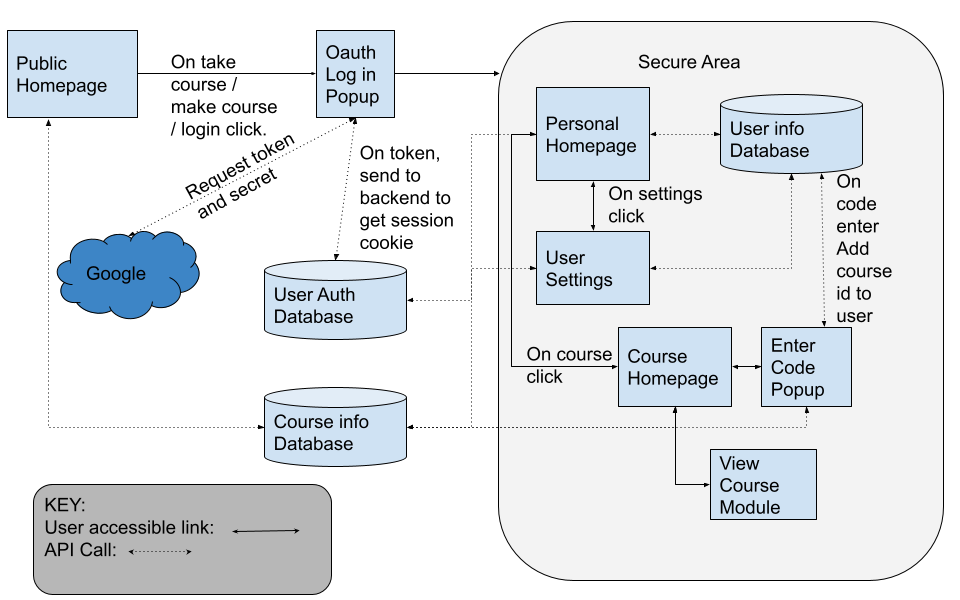
\includegraphics[width=\textwidth]{flow}
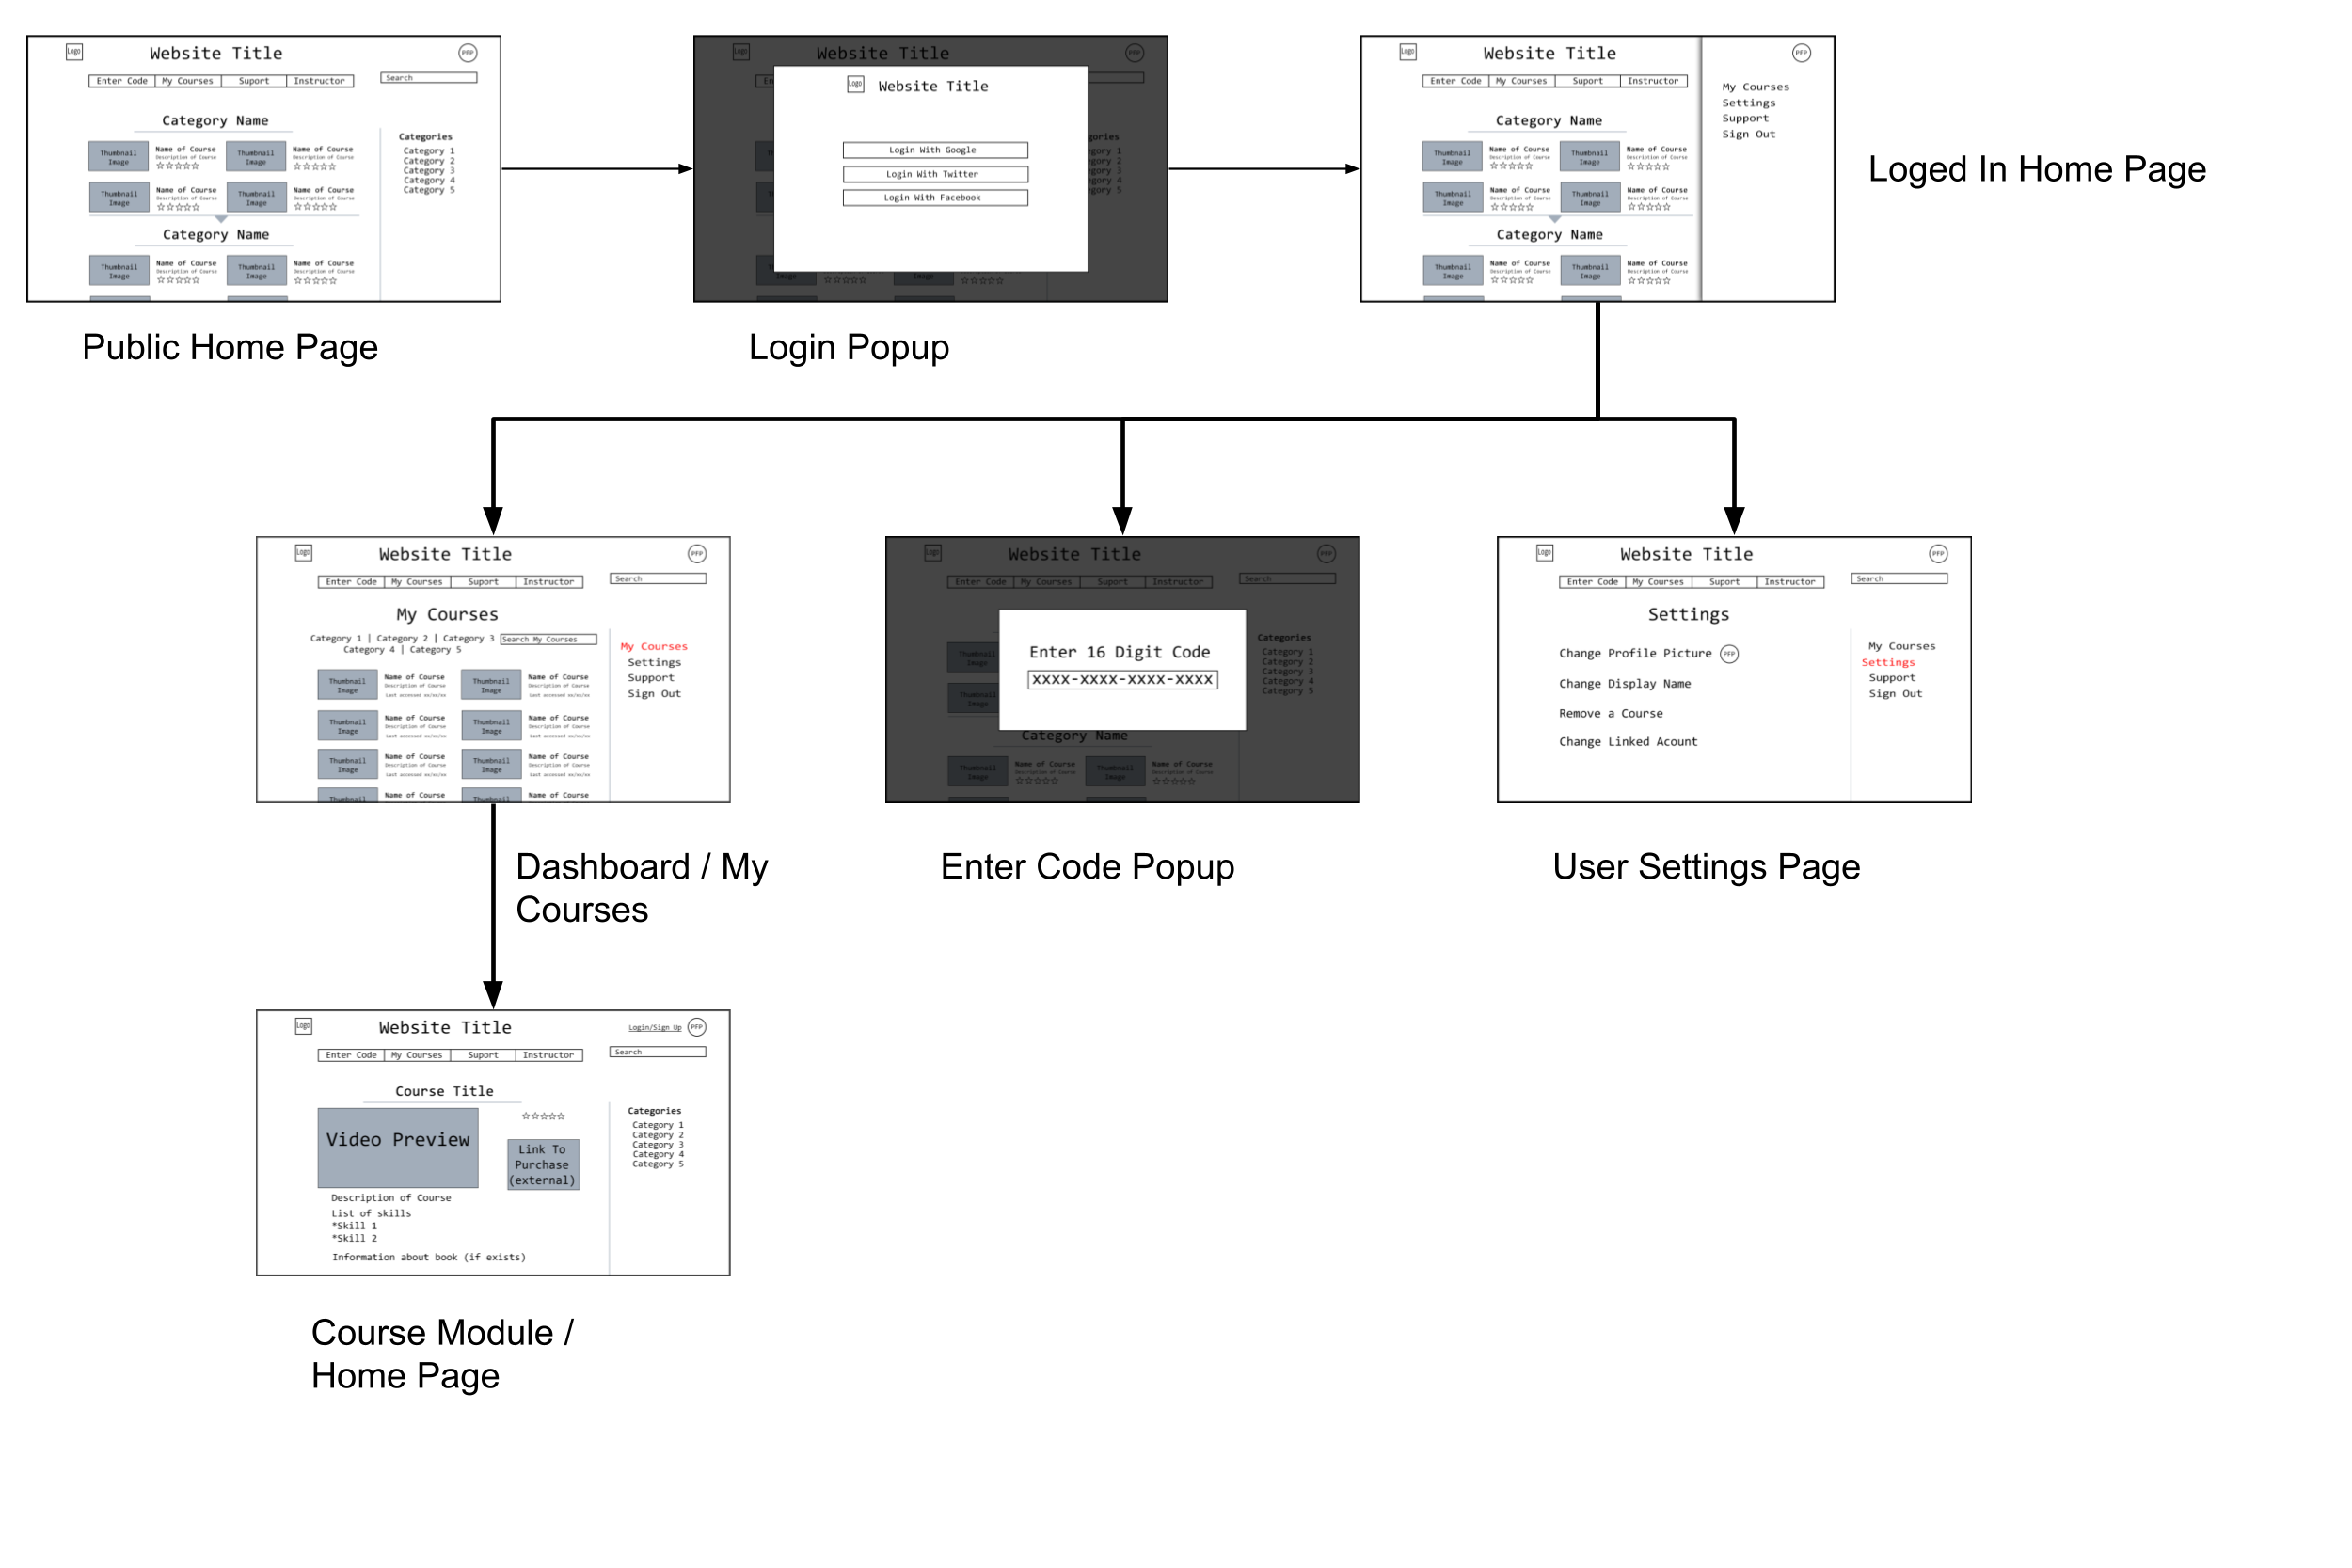
\includegraphics[width=\textwidth]{flow2}

\newpage

\paragraph{Public Homepage}
\vspace{\baselineskip}
\begin{itemize}
    \item \textbf{GET /}
    \begin{itemize}
        \item Link to open Login / sign up prompt.
        \item Listing of courses available.
        \item Pulls data from course data table.
        \item Has links to each courses' homepage.
        \item links to instructors and support are placeholders at professors request.
        \item User side search powered by js.
    \end{itemize}
\end{itemize}
\begin{figure}[h!]
    \caption{Mock-up of the public homepage.}
    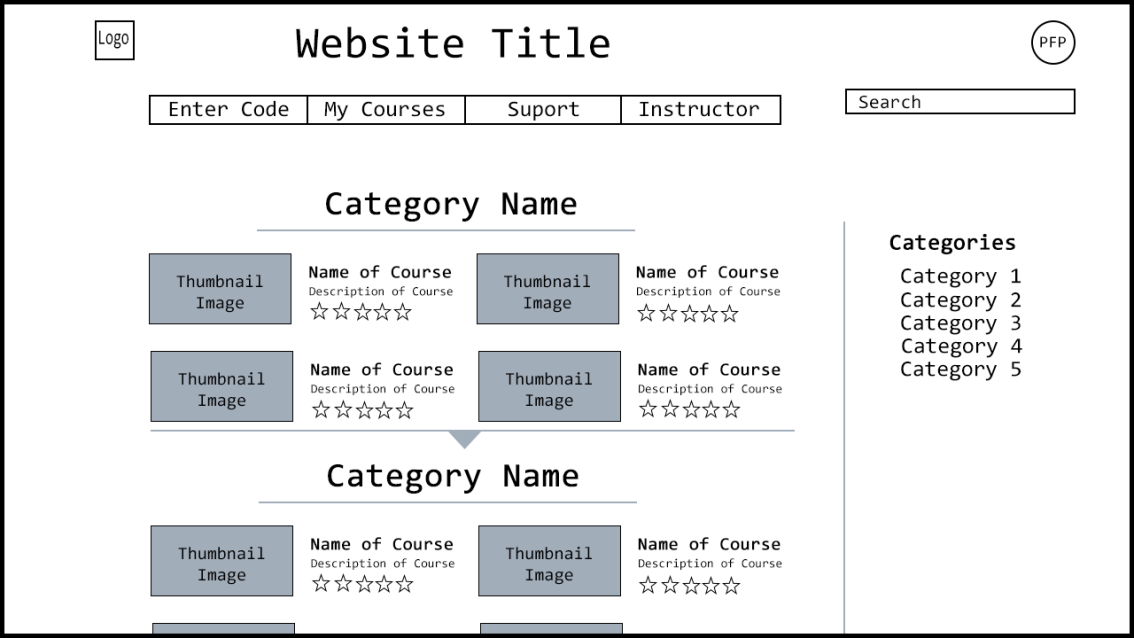
\includegraphics[width=\textwidth]{home_page}
\end{figure}
\begin{figure}[h!]
    \caption{Home page with categories extended.}
    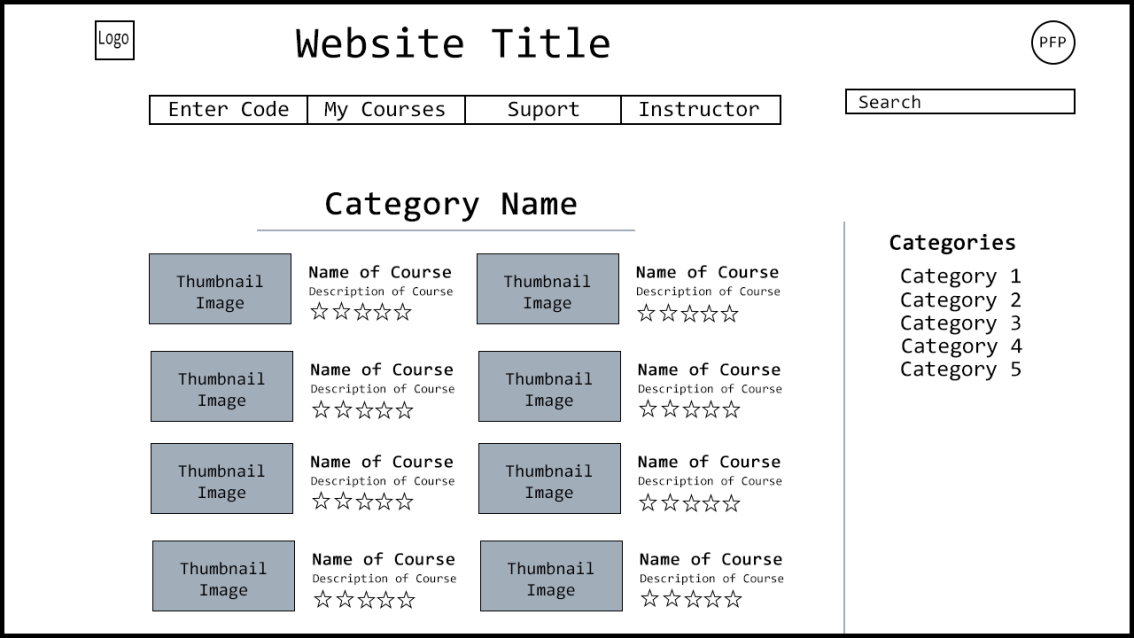
\includegraphics[width=\textwidth]{hompage_expanded}
\end{figure}
\begin{figure}[h!]
    \caption{Moc-up of home page with user logged in and user bar extended.
    This is replaced with a login prompt when user is not logged in.}
    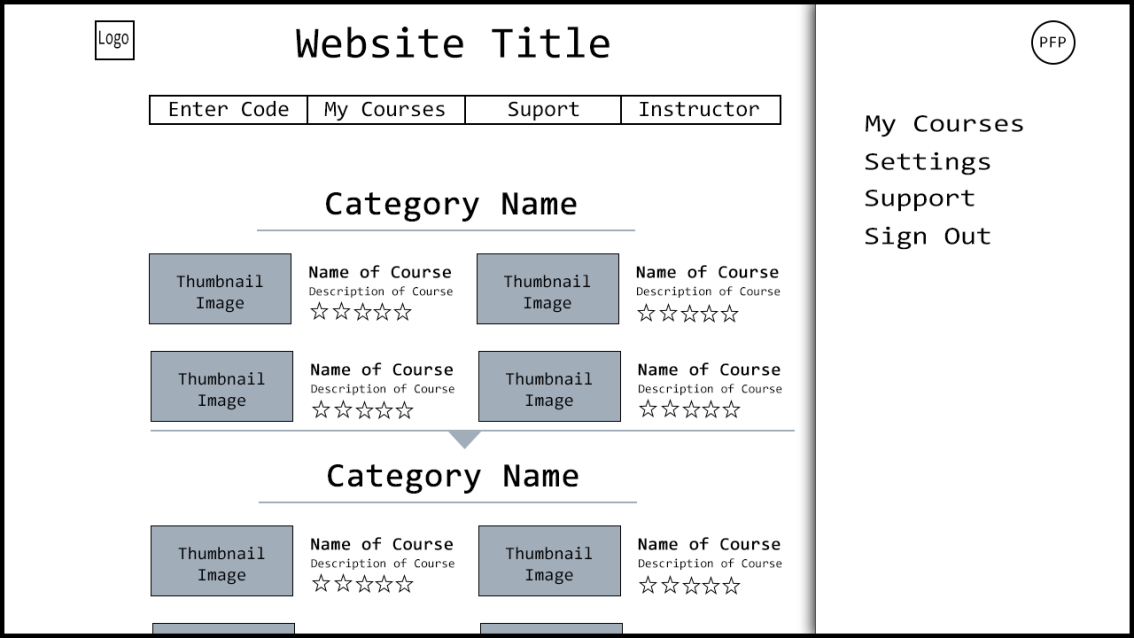
\includegraphics[width=\textwidth]{user_side_bar}
\end{figure}

\newpage

\paragraph{Login}

\vspace{\baselineskip}
\begin{itemize}
    \item \textbf{Login Popup}
    \begin{itemize}
        \item A button to sign in / sign up with OAuth2.
        \item A new, randomly generated state var to pass to oauth, this should
            be saved in a temp buffer server side.
        \item If a session cookie is passed with the request, void it in the
            auth database.
        \item If a session is passed with a redirect path param, set the
            redirect cookie to the given path so the user can be sent there
            after login.
        \item Caries out the rest of oauth.
    \end{itemize}
\end{itemize}
\begin{figure}[h!]
    \caption{Mock-up of the login popup.}
    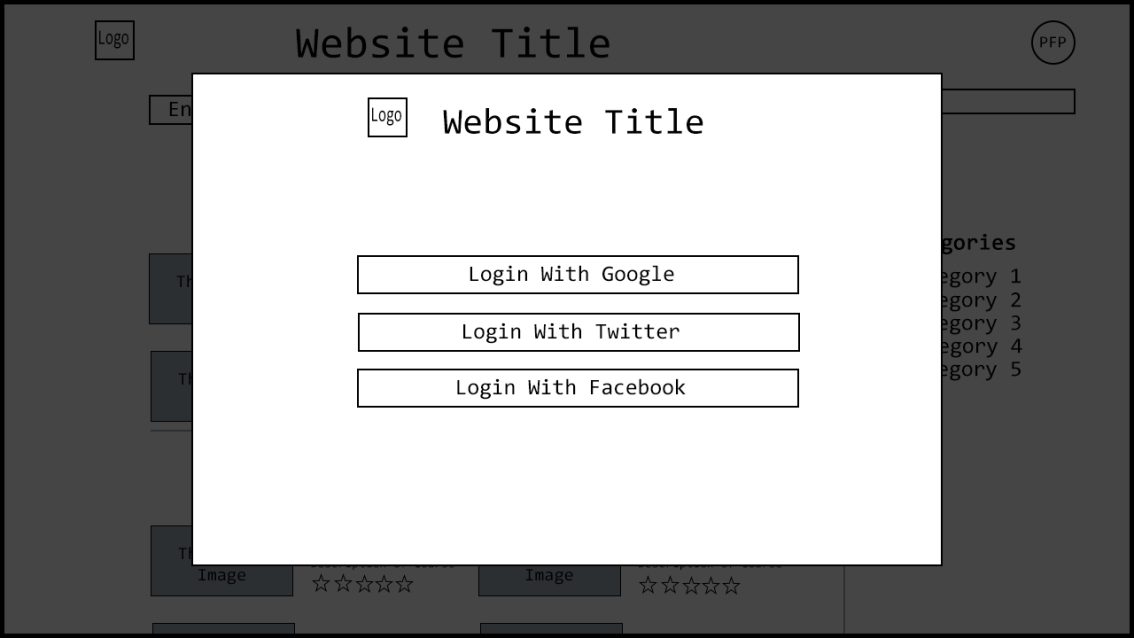
\includegraphics[width=\textwidth]{login}
\end{figure}

\newpage

%\paragraph{Oauth}\\
%\begin{itemize}
%    \item \textbf{GET /oauth?code=oauth code\&state=oauth state}
%    \begin{itemize}
%        \item Backend takes the code and state params and exchanges them for an auth token
%        \item Backend takes the code and state params and exchanges them for an auth tokenBackend should also ensure state is in that temp buffer from before, then remove it to protect from CSRF attacks
%        \item Backend takes the code and state params and exchanges them for an auth tokenBackend also adds a new user implicitly if they are not already in the db
%        \item Backend takes the code and state params and exchanges them for an auth tokenIf an auth token is received, Set the auth token as the new seBackend takes the code and state params and exchanges them for an auth tokenssion for that user in the auth table of the db, Returns a logged in page that redirects the user to whatever is set in the redirect cookie. Remember to clear cookie!
%        \item If one is not received, redirect user to /login after error message
%    \end{itemize}
%\end{itemize}
%\begin{figure}[h!]
%    \caption{Mock-up of the public homepage}
%    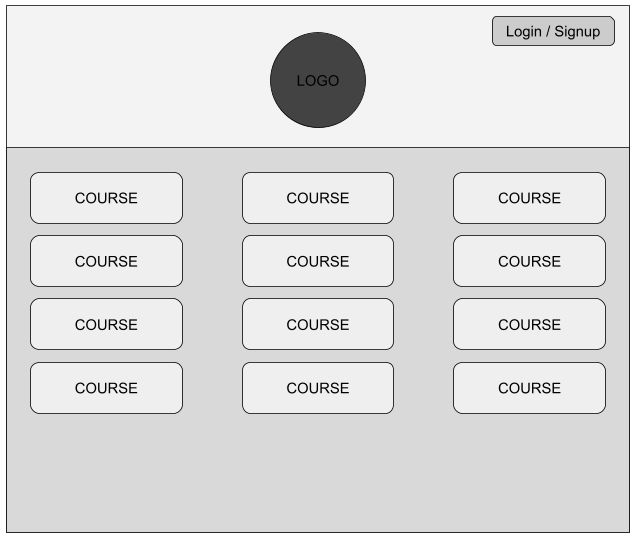
\includegraphics[width=\textwidth]{public_homepage}
%\end{figure}
%
%\newpage

\paragraph{Dashboard}
\vspace{\baselineskip}
\begin{itemize}
    \item \textbf{GET /dash}
        \begin{itemize}
        \item Page in secure area and backend needs to check for valid session
            token before serving page, if one is not found send the user to
                login.
        \item Backend Looks up session id to get user id. Takes user id and
            looks up user info and user course ids in the user info table of
                the db.
        \item Takes this info and serves a custom dashboard that has Links to
            courses and Links to user settings.
        \item links to instructors and support are placeholders at professors request.
        \item User side search powered by js.
    \end{itemize}
\end{itemize}
\begin{figure}[h!]
    \caption{Mock-up of the users dashboard}
    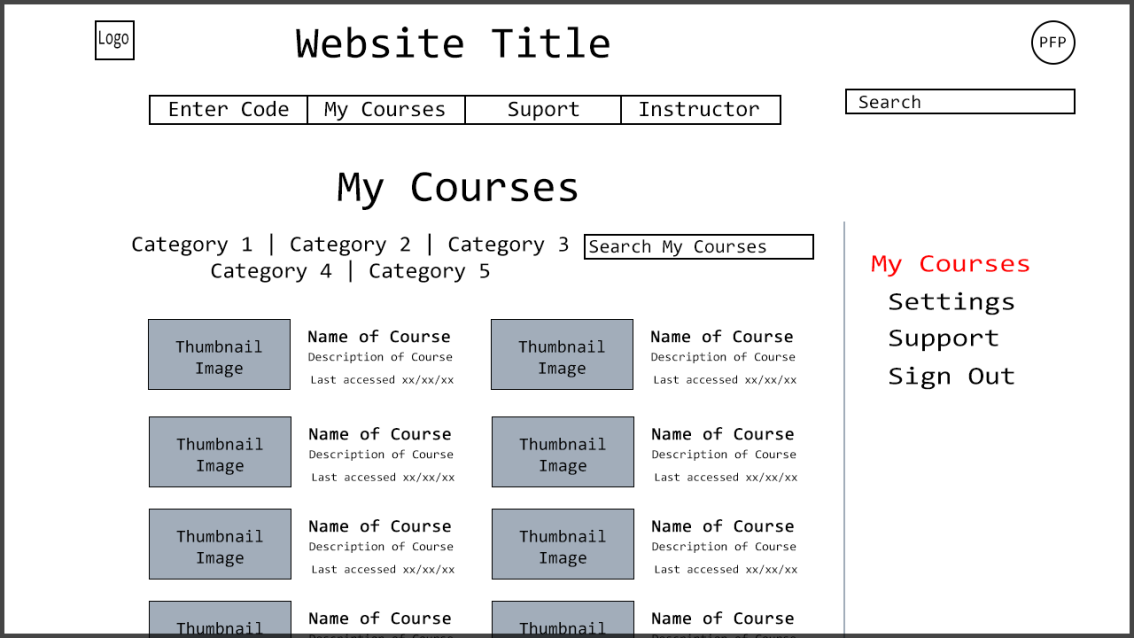
\includegraphics[width=\textwidth]{user_page}
\end{figure}
\begin{figure}[h!]
    \caption{In the users dash, the categories are only what categories of
    lessons the user has in their library, and the red means that's the active
    section.}
    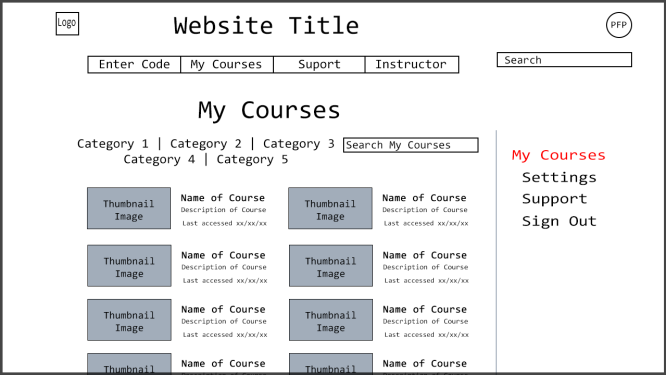
\includegraphics[width=\textwidth]{user_page_red}
\end{figure}

\newpage

\paragraph{User Settings}
\vspace{\baselineskip}
\begin{itemize}
    \item \textbf{GET /profile}
        \begin{itemize}
        \item Backend Looks up session id to get user id. Takes user id and
            looks up user info and user course ids in the user info table of
                the db.
        \item Takes this info and serves a custom dashboard that has The above info displayed, Input fields to modify mutable data, A save button that sends the forum data via POST to the same route.
    \end{itemize}
\item \textbf{POST /profile}
    \begin{itemize}
        \item Backend takes key:values passed in the body and updates user database with valid keys.
        \item Return the same page but with an updated prompt or an error message.
    \end{itemize}
\end{itemize}
\begin{figure}[h!]
    \caption{Mock-up of the main settings page.}
    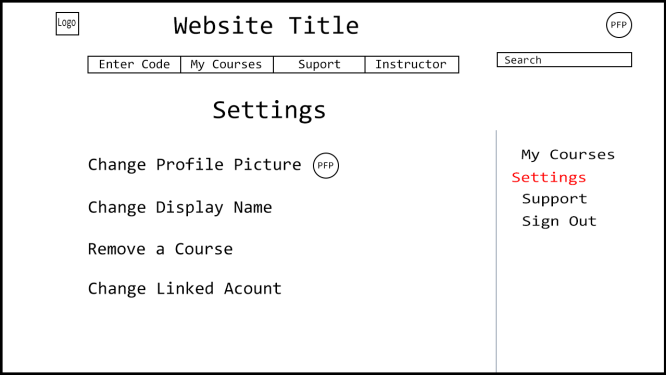
\includegraphics[width=\textwidth]{user_settings_page}
\end{figure}
\begin{figure}[h!]
    \caption{You can change the profile picture.}
    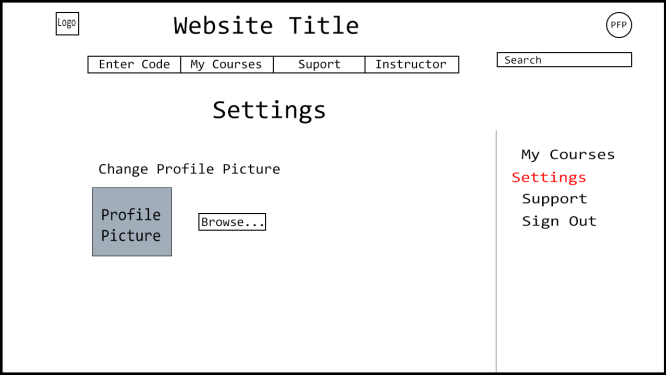
\includegraphics[width=\textwidth]{user_settings_page_pfp}
\end{figure}
\begin{figure}[h!]
    \caption{You can change your display name.}
    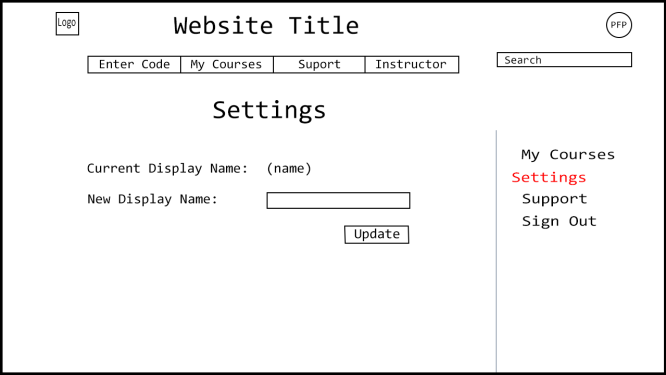
\includegraphics[width=\textwidth]{user_settings_page_display_name}
\end{figure}
\begin{figure}[h!]
    \caption{You can change many other things.}
    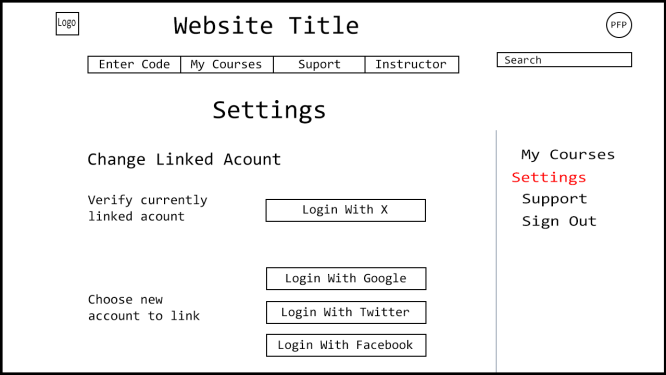
\includegraphics[width=\textwidth]{user_settings_page_change_account}
\end{figure}

\newpage

\paragraph{Course Homepage}
\vspace{\baselineskip}
\begin{itemize}
    \item \textbf{GET /c/home?id=course\_id}
        \begin{itemize}
        \item Page in secure area and backend needs to check for valid session
            token before serving page, if one is not found send the user to
                login.
        \item Backend Looks up the course id and returns details about the course.
        \item Lists a set of links to each of the courses modules.
        \item links to instructors and support are placeholders at professors request.
        \item User side search powered by js.
    \end{itemize}
\end{itemize}
\begin{figure}[h!]
    \caption{Mock-up of the course homepage}
    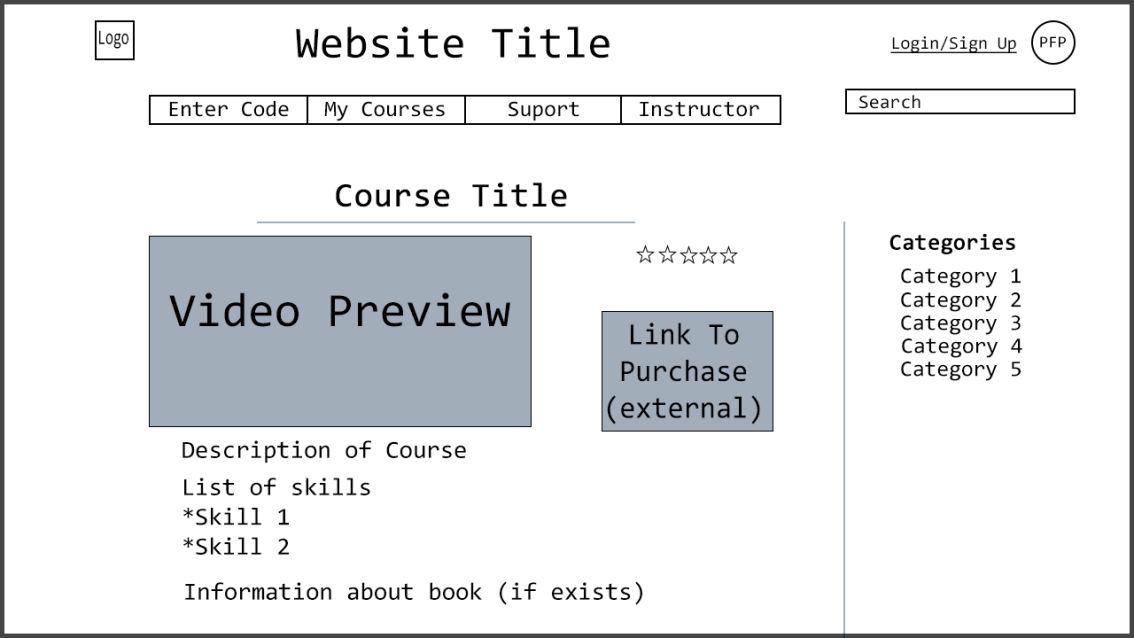
\includegraphics[width=\textwidth]{course_preview}
\end{figure}

\newpage

\paragraph{View Module}
\vspace{\baselineskip}
\begin{itemize}
    \item \textbf{GET /c/home?id=course\_id}
        \begin{itemize}
        \item Page in secure area and backend needs to check for valid session
            token before serving page, if one is not found send the user to
                login.
        \item Backend Looks up the course id and returns details about the course.
        \item Lists a set of links to each of the courses modules.
        \item links to instructors and support are placeholders at professors request.
        \item User side search powered by js.
    \end{itemize}
\end{itemize}
\begin{figure}[h!]
    \caption{Mock-up of the module view.}
    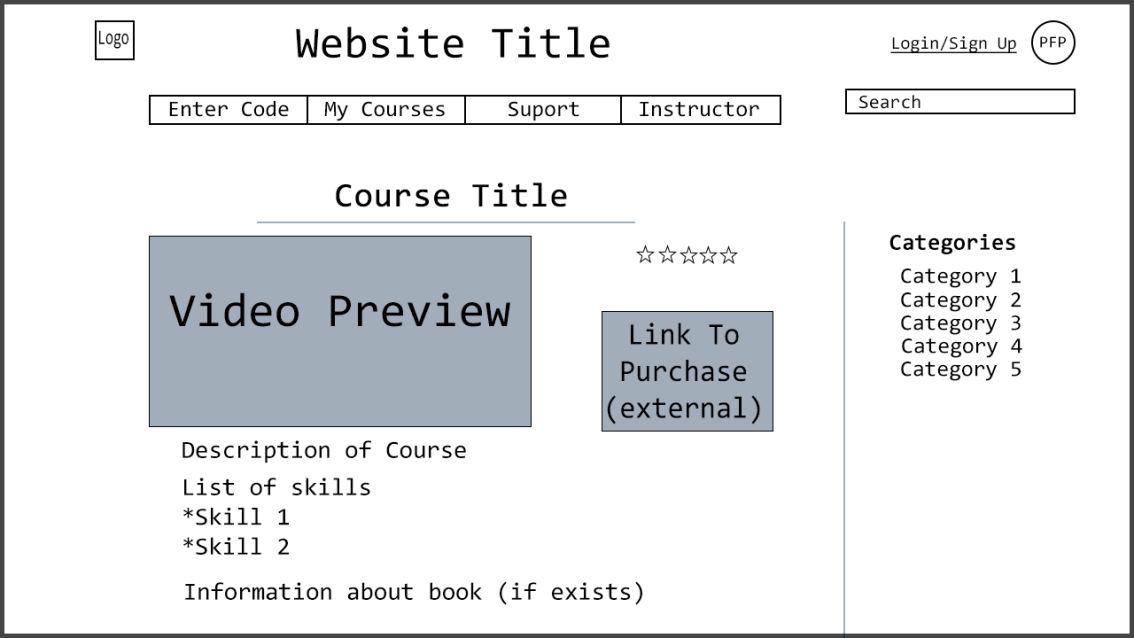
\includegraphics[width=\textwidth]{course_preview}
\end{figure}

\newpage

\paragraph{Enter Code}
\vspace{\baselineskip}
\begin{itemize}
    \item \textbf{Code Popup}
        \begin{itemize}
        \item Link to get code available on most pages.
        \item Backend Looks up the course id to validate code.
        \item If valid add user to the course table entry.
        \item links to instructors and support are placeholders at professors request.
        \item User side search powered by js.
    \end{itemize}
\end{itemize}
\begin{figure}[h!]
    \caption{Mock-up of the code popup.}
    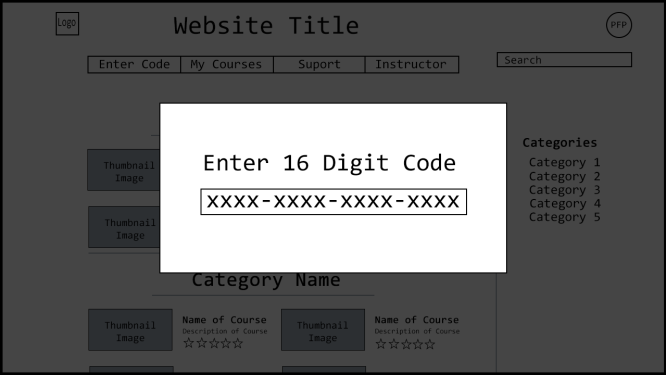
\includegraphics[width=\textwidth]{enter_code}
\end{figure}

\newpage

\paragraph{Mobile Content}
\vspace{\baselineskip}
\begin{figure}[h!]
    \caption{Mobile view of the video player.}
    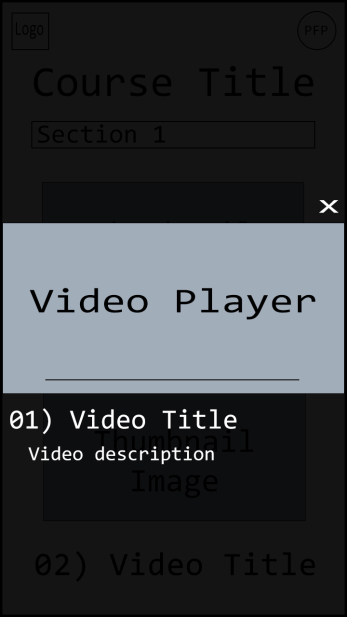
\includegraphics[height=10cm]{mobile_course_video}
\end{figure}
\begin{figure}[h!]
    \caption{Mobile view of course page.}
    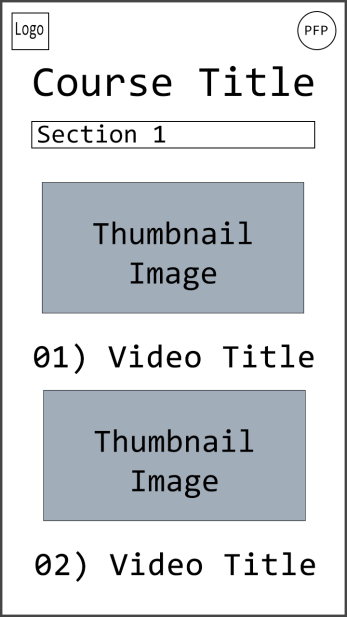
\includegraphics[height=10cm]{mobile_course_page}
\end{figure}

\clearpage

\section{ER Diagram}

The purpose of this section is to show how the database will be constructed to generate the various pages of the website. It includes the ER diagram, as well as a table for each node of the diagram explaining what variables are used in the table and how they relate to each other. 

\includepdf[pages=-,pagecommand={},width=1.5\textwidth]{er_diagram.pdf}

\subsection{Table Design}
\subsubsection{allUsers}
A table of all usesrs, used authenticate if the user is who they say they are and then to let the session know who is logged in and what they should have access to. This is linked to the courseOnwership and review table through the userID primary key. \\
\begin{tabular}{|m{1cm} | m{2.5cm} | m{1.5cm}| m{1cm} | m{1cm}| m{1cm} | m{1cm}| m{3.5cm}| }
  \hline
  Primary Key & Field Name & Data Type & Non-null & unique & binary & Foreign Key & Comments\\ 
  \hline
  x & userID & int(32) & x & x & & & Numeric ID for the user generated when a user is created, used to allow the user to change linked accounts\\
  \hline
   & linkedAccount & binary & x & x & x & & Information on the linked account used to log in\\
  \hline
\end{tabular}

\subsubsection{courseOwnership}
This table is an association table that associates each user with the courses that they own, while stating the last time the course was accessed in order to enable sorting. \\
\begin{tabular}{|m{1cm} | m{2cm} | m{1.5cm}| m{1cm} | m{1cm}| m{1cm} | m{1cm}| m{4cm}| }
  \hline
  Primary Key & Field Name & Data Type & Non-null & unique & binary & Foreign Key & Comments\\ 
  \hline
   & userID & int(32) & x & & & x & Numeric ID for the user\\
  \hline
   & courseID & int(32) & x & & & x & ID of each course the user owns\\
  \hline
   & courseID & timestamp & x & & & x & Time the user last accessed the course\\
  \hline
\end{tabular}

\subsubsection{courses}
A list of all the courses in the system, associated to the course content with the courseID field as a foriegn key and the primary key of this table.\\
\begin{tabular}{|m{1cm} | m{2.75cm} | m{2cm}| m{1cm} | m{1cm}| m{1cm} | m{1cm}| m{3cm}| }
  \hline
  Primary Key & Field Name & Data Type & Non-null & unique & binary & Foreign Key & Comments\\ 
  \hline
  x & courseID & int(32) & x & x & & & ID of the course within the system, generated automatically when the course is added to the database\\
  \hline
   & courseName & varchar(32) & x & & & & Name of the course presented to the user\\
  \hline
   & courseDesc & varchar(256) & & & & & Description about the course\\
  \hline
   & courseSkills & varchar(128) & & & & & List of skills that will be taught by the course\\
  \hline
   & bookDesc & varchar(128) & & & & & Description of the book related to the course, if there is one\\
  \hline
   & bookImageUrl & binary & & & x & & Link to the image of the book related to the course, if there is one\\
  \hline
   & courseImageURL & binary & & & x & & Link to the image featured for the course\\
  \hline
   & previewVideoURL & binary & & & x & & Link to the preview embedded in the preview of it.\\
  \hline
   & imageURL & binary & & & x & & link to the image\\
  \hline
\end{tabular}

\subsubsection{categoryAssociations}
an association table with two foreign keys linking them to the course table and category table to assoiciate courses and categories for the sorting of courses. \\
\begin{tabular}{|m{1cm} | m{2cm} | m{1.5cm}| m{1cm} | m{1cm}| m{1cm} | m{1cm}| m{4cm}| }
  \hline
  Primary Key & Field Name & Data Type & Non-null & unique & binary & Foreign Key & Comments\\ 
  \hline
   & courseID & int(32) & x & & & x & Id of the course associated with the category\\
  \hline
   & categoryID & int(16) & x & & & x & ID of the category associated with the course\\
  \hline
\end{tabular}

\subsubsection{categoryNames}
an end table that simply contains each unique category and its name so that it can be retrieved by the primary key of courseID whenever the category needs to have it's name displayed. \\
\begin{tabular}{|m{1cm} | m{2cm} | m{1.5cm}| m{1cm} | m{1cm}| m{1cm} | m{1cm}| m{4cm}| }
  \hline
  Primary Key & Field Name & Data Type & Non-null & unique & binary & Foreign Key & Comments\\ 
  \hline
  x & categoryID & int(16) & x & & & & Category ID associated above\\
  \hline
   & categoryName & varchar(16) & x & & & & Name of the category\\
  \hline
\end{tabular}

\subsubsection{reviews}
A table of reviews, where each course and user combination serves together as the primary key as each user can only leave one review on each course. When aggregating the courseID or userID is used as a foriegn key to associate courses with reviews or a user with their reviews. \\
\begin{tabular}{|m{1cm} | m{2cm} | m{2.0cm}| m{1cm} | m{1cm}| m{1cm} | m{1cm}| m{3.5cm}| }
  \hline
  Primary Key & Field Name & Data Type & Non-null & unique & binary & Foreign Key & Comments\\ 
  \hline
  x & courseID & int(32) & x & & & x & ID of the course the rating is for\\
  \hline
   & rating & decimal(4) & x & & & & Rating between 1-5\\
  \hline
   & review & varchar(128) & & & & & Text of the review\\
  \hline
  x & userID & int(32) & & & & x & Id of the user who wrote the review\\
  \hline
\end{tabular}

\subsubsection{courseSections}
An association table for each individual course that details the list of sections and what content items are associated with that section. The courseID is used as a forign key so that the course knows what sections it has and the contentID Foreign key is used to associate the name and order of the section to the individual piece of content. \\
\begin{tabular}{|m{1cm} | m{2cm} | m{2cm}| m{1cm} | m{1cm}| m{1cm} | m{1cm}| m{3.5cm}| }
  \hline
  Primary Key & Field Name & Data Type & Non-null & unique & binary & Foreign Key & Comments\\ 
  \hline
   & courseID & int(32) & x & & & x & Id of the course this content item is associated with\\
  \hline
   & contentID & int(32) & x & & & x & ID of the content associated with this course\\
  \hline
   & sectionName & varchar(16) & & & & & Number of the section this is associated with\\
  \hline
   & sectionOrder & int(8) & & & & & Order in which the section should appear when generating the course\\
  \hline
\end{tabular}

\subsubsection{courseContent}
The table for each course containing every individual piece of content. Each piece of content can be associated with the contentID primary key to a tag in the contentTags table. Each piece of content can contain a main and extra piece of content with the extra content being not required.\\
\begin{tabular}{|m{1cm} | m{2.7cm} | m{2cm}| m{.8cm} | m{.8cm}| m{.8cm} | m{.8cm}| m{3.5cm}| }
  \hline
  Primary Key & Field Name & Data Type & Non-null & unique & binary & Foreign Key & Comments\\ 
  \hline
  x & contentID & int(32) & x & & & & ID of this content section, automatically generated when added to the system\\
  \hline
   & mainContentType & int(4) & x & & & & Type of content linked in this table, either a pdf, video, or audio file, denoted by 0,1,2\\
  \hline
   & mainContentURL & binary & x & & & & The link to the content on the server\\
  \hline
   & mainContentName & varchar(16) & x & & & & Title of the content for the user to click on\\
  \hline
   & contentDesc & varchar(128) & & & & & Description of this content\\
  \hline
   & extraContentType & int(4) & & & & & Type of extra content linked in this table, either a pdf, video, or audio file, denoted by 0,1,2\\
  \hline
   & extraURL & binary & & & & & The link to the extra content on the server\\
  \hline
   & extraName & varchar(16) & & & & & Title of the extra content for the user to click on\\
  \hline
   & contentOrder & int(16) & x & & & & The order in which the content should be presented to the user on the generated page\\
  \hline
\end{tabular}

\subsubsection{contentTags}
An association table that associates each piece of content to the tags it goes with using the contentID as the foreign key to associate with.\\
\begin{tabular}{|m{1cm} | m{2cm} | m{1.5cm}| m{1cm} | m{1cm}| m{1cm} | m{1cm}| m{4cm}| }
  \hline
  Primary Key & Field Name & Data Type & Non-null & unique & binary & Foreign Key & Comments\\ 
  \hline
   & contentID & int(32) & x & & & x & The id of the content the extra is associated with\\
  \hline
   & tagID & int(16) & x & & & x & The id of the tag, within this course\\
  \hline
\end{tabular}

\subsubsection{tagNames}
A table with the primary key being the tag ID to list each unique tag as well as it's name within the system.\\
\begin{tabular}{|m{1cm} | m{2cm} | m{1.5cm}| m{1cm} | m{1cm}| m{1cm} | m{1cm}| m{4cm}| }
  \hline
  Primary Key & Field Name & Data Type & Non-null & unique & binary & Foreign Key & Comments\\ 
  \hline
  x & tagID & int(16) & x & & & & The id of the tag only within this course, generated when added to the table\\
  \hline
   & tagName & varchar(16) & & & & & the name of the tag only within this course\\
  \hline
\end{tabular}

\subsubsection{Sessions}
While session data is primarily managed with serverlet sessions, this table is used to maintain a log of logons for audit purposes. It is indexed by a unique session ID and with the foreign key of the userID of the user the log on was linked to. The cookie used and when it was valid for is tracked to identify rouge sessions.\\
\begin{tabular}{|m{1cm} | m{2cm} | m{1.5cm}| m{1cm} | m{1cm}| m{1cm} | m{1cm}| m{4cm}| }
  \hline
  Primary Key & Field Name & Data Type & Non-null & unique & binary & Foreign Key & Comments\\ 
  \hline
  x & sessionID & int(32) & x & x & & & Used to index sessions.\\
  \hline
   & userID & int(32) & x & & & x & The account that the session is tied to.\\
  \hline
   & sessionCookie & int(32) & x & x & & & The session cookie issued.\\
  \hline
   & grantDate & int(32) & x &  & &  & Time Session was granted (unix time).\\
  \hline
   & endDate & int(32) & x &  & &  & Time Session expires (unix time).\\
  \hline
\end{tabular}

\section{System Architecture}
\subsection{5.a}
    The structure of our site folows a MCV system higlighted in the figure below.
\begin{figure}[h!]
    \caption{MCV flow of Sesha.}
    \includegraphics[height=10cm]{mcv}
\end{figure}
\subsection{5.b}
    To acchieve the goals of Sesha we implemented two objects for our model: a User and Course object.
    \begin{enumerate}
        \item \textit{Object}
            \begin{enumerate}
                \item Tracks user credentials for authentication.
                \item Contians the courseIDs of of courses owned by the user.
            \end{enumerate}
        \item \textit{Course}
            \begin{enumerate}
                \item Made up of organized sections.
                \item Sections are filled with rich content.
                \item Courses also contain metadata.
                \item Metadat allows for catagory sorting and the access code feature.
            \end{enumerate}
    \end{enumerate}
    The controler is simple but robust, taking the requested view as the "action" parameter and sanatizing the all other paramters. Once sanatized, if all inputs are valid, the requested view is generated.
    
    Views are generated in via a pipeline. First the header and footer is generated, including sitewide scripts and css. Then an authntication check is made. If the user is loged in and has permision to see the requested view they are directed to the requested view. Otherwise, they are redirected to the login screen. Since the settings are tied into the authenitcation system, this is where that redirect is also perforemd. A visual representation of each of the final views can be seen in the system snapshot section. The general idea of these remianing views beingn ways to view courses at varing levels of grainularity. With the homepage you can see all avalable courses; with the myCourses view you can see owned courses; with the preview page you can see an overview of the course; and finaly, with the view page you can actualy interact with the content of a course. Each of these levels are accesable from any of the others asuuming the user has permisions for the course in question.

\section{System Snapshot}

\includepdf[pages=-,pagecommand={},width=2\textwidth,height=1.5\textheight]{system snapshot.pdf}

\section{conclusion}

\subsection{Project as it is}
Currently the project has this functionality  
\begin{itemize}
  \item A home page, with the ability to search for courses by text and by category
  \item The ability to expand each section to display more courses
  \item The ability to preview each of theses courses, with a video and then some details, and then purchase the course, adding it to your account when you log in
  \item A login system and account creation system
  \item The ability to log out of the system
  \item A code redemption system
  \item The ability to view a course, generated with videos and PDF files
  \item The ability to switch sections in a course.
  \item The ability to view what courses you own, search within that by text and category
  \item Automatic sorting of courses in my courses by when the user accessed them
\end{itemize}
\subsection{future works}
In the future these should be added:
\begin{itemize}
    \item A rating system should be added.
    \item A way to generate statistics about how many people own a courses, what the ratings are, etc, in order to customize the home page, possibly with personal customization for courses similar to those the user owns
    \item Courses should not be duplicated in multiple sections on the main page 
    \item Courses on the main page should be loaded in upon pressing the (show more) button instead of all being loaded upon the page load.
    \item The ability to upload a course, as well as fine instructor controls
    \item the login page should be improved to redirect correctly every time, as there are currently two cases in which it fails (entering a correct code then logging in, purchasing a course without an established account)
    \item The servlet needs to be made so that it displays a unique url for each of the pages, currently whenever in the servlet it just displays the servlet.
    \item the design needs a massive amount of work to not look like a template site
    \item Account management features need to be added
\end{itemize}


\end{document}
